% vim: set textwidth=120:

% Example CV based on the 1.5-column-cv template. Main features:
% * uses the Roboto font family and IcoMoon icon set;
% * doesn't use colours, different font weights are used instead for styling;
% * because the CV fits on one page, header and footer is empty, since there isn't much useful info to put there;
% * includes a photo.
\documentclass[a4paper,10pt]{article}

% package imports
% ---------------

\usepackage[british]{babel} % for correct language and hyphenation and stuff
\usepackage{calc}           % for easier length calculations (infix notation)
\usepackage{enumitem}       % for configuring list environments
\usepackage{fancyhdr}       % for setting header and footer
\usepackage{fontspec}       % for fonts
\usepackage{geometry}       % for setting margins (\newgeometry)
\usepackage{graphicx}       % for pictures
\usepackage{microtype}      % for microtypography stuff
\usepackage{xcolor}         % for colours
\usepackage{hyperref}       % references

\usepackage{verbatim} % comment paragraphs

% margin and column widths
% ------------------------

% margins
\newgeometry{left=15mm,right=15mm,top=15mm,bottom=15mm}

% width of the gap between the left and right column
\newlength{\cvcolumngapwidth}
\setlength{\cvcolumngapwidth}{3.5mm}

% left column width
\newlength{\cvleftcolumnwidth}
\setlength{\cvleftcolumnwidth}{44.5mm}

% right column width
\newlength{\cvrightcolumnwidth}
\setlength{\cvrightcolumnwidth}{\textwidth-\cvleftcolumnwidth-\cvcolumngapwidth}

% Set paragraph indentation to 0, because it screws up the whole layout otherwise
\setlength{\parindent}{0mm}


% style definitions
% -----------------
% style categories explanation:
% * \cvnameXXX is used for the name;
% * \cvsectionXXX is used for section names (left column, accompanied by a horizontal rule);
% * \cvtitleXXX is used for job/education titles (right column);
% * \cvdurationXXX is used for job/education durations (left column);
% * \cvheadingXXX is used for headings (left column);
% * \cvmainXXX (and \setmainfont) is used for main text;
% * \cvruleXXX is used for the horizontal rules denoting sections.

% font families
\defaultfontfeatures{Ligatures=TeX} % reportedly a good idea, see https://tex.stackexchange.com/a/37251

\newfontfamily{\cvnamefont}{Roboto Medium}
\newfontfamily{\cvsectionfont}{Roboto Medium}
\newfontfamily{\cvtitlefont}{Roboto Regular}
\newfontfamily{\cvdurationfont}{Roboto Light Italic}
\newfontfamily{\cvheadingfont}{Roboto Regular}
\setmainfont{Roboto Light}[ItalicFont=Roboto-LightItalic]
% colors
\definecolor{cvnamecolor}{HTML}{000000}
\definecolor{cvsectioncolor}{HTML}{000000}
\definecolor{cvtitlecolor}{HTML}{000000}
\definecolor{cvdurationcolor}{HTML}{000000}
\definecolor{cvheadingcolor}{HTML}{000000}
\definecolor{cvmaincolor}{HTML}{000000}
\definecolor{cvrulecolor}{HTML}{000000}

\color{cvmaincolor}

% styles
\newcommand{\cvnamestyle}[1]{{\Large\cvnamefont\textcolor{cvnamecolor}{#1}}}
\newcommand{\cvsectionstyle}[1]{{\normalsize\cvsectionfont\textcolor{cvsectioncolor}{#1}}}
\newcommand{\cvtitlestyle}[1]{{\large\cvtitlefont\textcolor{cvtitlecolor}{#1}}}
\newcommand{\cvdurationstyle}[1]{{\small\cvdurationfont\textcolor{cvdurationcolor}{#1}}}
\newcommand{\cvheadingstyle}[1]{{\normalsize\cvheadingfont\textcolor{cvheadingcolor}{#1}}}


% inter-item spacing
% ------------------

% vertical space after personal info and standard CV items
\newlength{\cvafteritemskipamount}
\setlength{\cvafteritemskipamount}{5mm plus 1.25mm minus 1.25mm}

% vertical space after sections
\newlength{\cvaftersectionskipamount}
\setlength{\cvaftersectionskipamount}{2mm plus 0.5mm minus 0.5mm}

% extra vertical space to be used when a section starts with an item with a heading (e.g. in the skills section),
% so that the heading does not follow the section name too closely
\newlength{\cvbetweensectionandheadingextraskipamount}
\setlength{\cvbetweensectionandheadingextraskipamount}{1mm plus 0.25mm minus 0.25mm}


% intra-item spacing
% ------------------

% vertical space after name
\newlength{\cvafternameskipamount}
\setlength{\cvafternameskipamount}{3mm plus 0.75mm minus 0.75mm}

% vertical space after personal info lines
\newlength{\cvafterpersonalinfolineskipamount}
\setlength{\cvafterpersonalinfolineskipamount}{2mm plus 0.5mm minus 0.5mm}

% vertical space after titles
\newlength{\cvaftertitleskipamount}
\setlength{\cvaftertitleskipamount}{1mm plus 0.25mm minus 0.25mm}

% value to be used as parskip in right column of CV items and itemsep in lists (same for both, for consistency)
\newlength{\cvparskip}
\setlength{\cvparskip}{0.5mm plus 0.125mm minus 0.125mm}

% set global list configuration (use parskip as itemsep, and no separation otherwise)
\setlist{parsep=0mm,topsep=0mm,partopsep=0mm,itemsep=\cvparskip}


% CV commands
% -----------

% creates a "personal info" CV item with the given left and right column contents, with appropriate vertical space after
% @param #1 left column content (should be the CV photo)
% @param #2 right column content (should be the name and personal info)
\newcommand{\cvpersonalinfo}[2]{
    % left and right column
    \begin{minipage}[t]{\cvleftcolumnwidth}
        \vspace{0mm} % XXX hack to align to top, see https://tex.stackexchange.com/a/11632
        \raggedleft #1
    \end{minipage}% XXX necessary comment to avoid unwanted space
    \hspace{\cvcolumngapwidth}% XXX necessary comment to avoid unwanted space
    \begin{minipage}[t]{\cvrightcolumnwidth}
        \vspace{0mm} % XXX hack to align to top, see https://tex.stackexchange.com/a/11632
        #2
    \end{minipage}

    % space after
    \vspace{\cvafteritemskipamount}
}

% typesets a name, with appropriate vertical space after
% @param #1 name text
\newcommand{\cvname}[1]{
    % name
    \cvnamestyle{#1}

    % space after
    \vspace{\cvafternameskipamount}
}

% typesets a line of personal info beginning with an icon, with appropriate vertical space after
% @param #1 parameters for the \includegraphics command used to include the icon
% @param #2 icon filename
% @param #3 line text
\newcommand{\cvpersonalinfolinewithicon}[3]{
    % icon, vertically aligned with text (see https://tex.stackexchange.com/a/129463)
    \raisebox{.5\fontcharht\font`E-.5\height}{\includegraphics[#1]{#2}}
    % text
    #3

    % space after
    \vspace{\cvafterpersonalinfolineskipamount}
}

% creates a "section" CV item with the given left column content, a horizontal rule in the right column, and with
% appropriate vertical space after
% @param #1 left column content (should be the section name)
\newcommand{\cvsection}[1]{
    % left and right column
    \begin{minipage}[t]{\cvleftcolumnwidth}
        \raggedleft\cvsectionstyle{#1}
    \end{minipage}% XXX necessary comment to avoid unwanted space
    \hspace{\cvcolumngapwidth}% XXX necessary comment to avoid unwanted space
    \begin{minipage}[t]{\cvrightcolumnwidth}
        \textcolor{cvrulecolor}{\rule{\cvrightcolumnwidth}{0.3mm}}
    \end{minipage}

    % space after
    \vspace{\cvaftersectionskipamount}
}

% creates a standard, multi-purpose CV item with the given left and right column contents, parskip set to cvparskip
% in the right column, and with appropriate vertical space after
% @param #1 left column content
% @param #2 right column content
\newcommand{\cvitem}[2]{
    % left and right column
    \begin{minipage}[t]{\cvleftcolumnwidth}
        \raggedleft #1
    \end{minipage}% XXX necessary comment to avoid unwanted space
    \hspace{\cvcolumngapwidth}% XXX necessary comment to avoid unwanted space
    \begin{minipage}[t]{\cvrightcolumnwidth}
        \setlength{\parskip}{\cvparskip} #2
    \end{minipage}

    % space after
    \vspace{\cvafteritemskipamount}
}

% typesets a title, with appropriate vertical space after
% @param #1 title text
\newcommand{\cvtitle}[1]{
    % title
    \cvtitlestyle{#1}

    % space after
    \vspace{\cvaftertitleskipamount}
    % XXX needs to subtract cvparskip here because it is automatically inserted after the title "paragraph"
    \vspace{-\cvparskip}
}


% header and footer
% -----------------

% set empty header and footer
\pagestyle{empty}



% preamble end/document start
% ===========================

\begin{document}


% personal info
% -------------

\cvpersonalinfo{
    % photo
    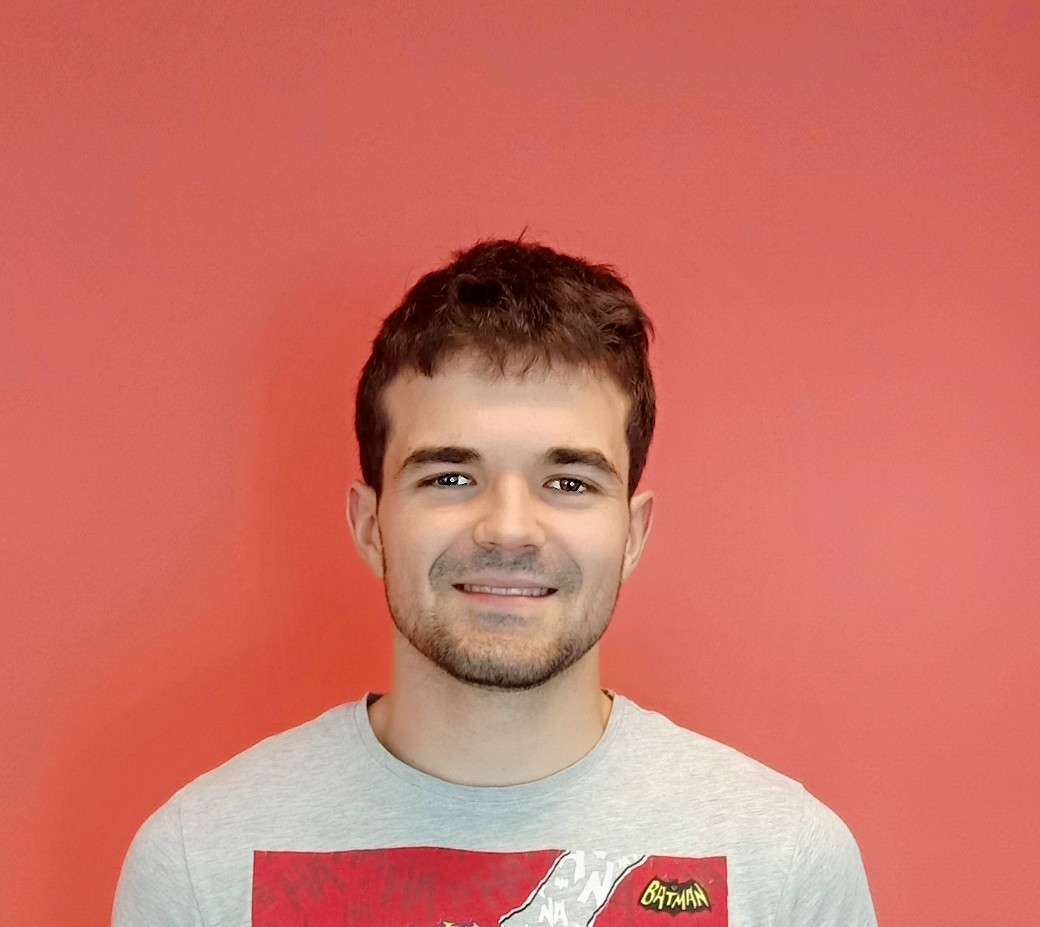
\includegraphics[height=42mm]{foto.jpg}
}{
    % name
    \cvname{Pau Torres i Bravo}

    % address
    \cvpersonalinfolinewithicon{height=4mm}{072-location.pdf}{
        Avinguda Dosrius 42, Can Massuet-El Far (Dosrius)
    }

    % phone number
    \cvpersonalinfolinewithicon{height=4mm}{067-phone.pdf}{
        +34 654 71 45 27
    }

    % email address
    \cvpersonalinfolinewithicon{height=4mm}{070-envelop.pdf}{
        entimos34@gmail.com
    }

    % LinkedIn account
    \cvpersonalinfolinewithicon{height=4mm}{458-linkedin.pdf}{
        Pau Torres i Bravo
    }
    
    % Github account
    \cvpersonalinfolinewithicon{height=4mm}{github.png}{
        pautib
    }

    % date of birth
    Born 2 August 1994
}


% work experience
% ---------------

\cvsection{WORK EXPERIENCE}

% Company 4

\cvitem{
    \cvdurationstyle{July 2023 - 
    }
}{
    \cvtitle{Senior Software Engineer}
    
    IGT, Prat de Llobregat 
    \vspace{5pt}
    \begin{itemize}[leftmargin=*]
        \item \textbf{Description:} Adding more responsibilities to my role in IGT. Taking care of the back-end development of small projects by myself, performing software design documentation, and evaluating the time needed to implement a project for the Business Analyst and management team.
    \end{itemize}
}

\cvitem{
    \cvdurationstyle{July 2021 - June 2023}
}{
    \cvtitle{Software Engineer}
    
    IGT, Prat de Llobregat 
    \vspace{5pt}
    \begin{itemize}[leftmargin=*]
        \item \textbf{Description:} As part of the middleware team, I contribute to developing and improving the services connecting our customers with the Aurora transaction engine at IGT. My daily tasks involve solving bugs on our lottery projects and customizing our baseline products according to our clients's specifications. I am also in charge of creating API simulations to fasten the job of our QA peers and write technical or functional documentation about the software, either for internal or business purposes.
        \vspace{5pt}
        \item \textbf{Achievements:} In charge of the middle-ware design and implementation of a project for Portugal's lottery within a considerably restrictive time range, providing excellent maintainable code reused in posterior projects of the same site. This project involved the creation of Spring classes to equip one of our back-end products with the ability to send requests to Portugal's lottery infrastructure and track all the information being sent and received through daily log files.
    \end{itemize}
}

% Company 3

\cvitem{
    \cvdurationstyle{May 2019 - July 2021}
}{
    \cvtitle{IT consultant}
    
    Better Consultants, Barcelona 
    \vspace{5pt}
    \begin{itemize}[leftmargin=*]
        \item \textbf{Description:} Maintenance and development of the web application used by Barcelona City Council to estimate the imputation of city planning fines. It involves resolving incidents in the database in case the users cannot solve them with the application and the correction of bugs by modifying Java code. Other tasks consist of documenting the changes made in the app and participating in meetings with the team, project manager, or client to discuss current problems or future improvements.\newline

        Tech stack: Oracle SQL, Java 5, Eclipse IDE, Microsoft Teams, Jira, and Kibana. The main tool used on the job is Oracle SQL to make queries on the application database or create new views, updating or inserting fields in production if the incidents require it. Creation of reports to inform about new updates made on the application, preparing tables and diagrams for presentations where we discussed the volume of incidents created and resolved periodically.
        % Give support when it comes to testing the changes made in the app of this project and other Java projects of the company. 
        \vspace{5pt}
        \item \textbf{Achievements:} My major contributions to the project involved not only being compromised with the client by resolving their incidents apace as they send them but also in providing final software solutions to some endemic problems the application had from its first release. Those problems generated recurrent incidences for our department to take over and programming a solution required a proper understanding of the flow of the data in the app, both functional and technical. To highlight, the development of a functionality that allows users to move steps back inside a fine procedure to redo tasks finished incorrectly (without having to send us a task to do it for them). % Some others: Improving the way inspection violations are shown on the screen, a core task inside the app, and modifying a batch process that collects the documentation of a fine procedure in a single document by making its index dynamic so users can access each concatenated document by clicking its register on the index. 
        Providing an automatized solution to this and other problems diminished by more than half the volume of incidences we received per month compared to when I started working in the company. The department won the trust of our customers to carry out more development tasks in the future.
    \end{itemize}
}

% Company 2

\cvitem{
    \cvdurationstyle{August 2018 - March 2019
   \hspace{15pt} (6 months)}
}{
    \cvtitle{Research assistant}
    
    The University of Auckland, Auckland  
    \vspace{5pt}
    \begin{itemize}[leftmargin=*]
        \item \textbf{Description:} Development of research on phylogenetics. My duty was to help in a lab under the supervision of doctors Fábio Kuriki Mendes and Alexei J. Drummond in understanding mathematical models applied to phylogenetics and implementing them in \href{https://www.beast2.org}{BEAST}, a Java platform for Bayesian phylogenetic analysis created and maintained by the department of computer science at the University of Auckland. Contribution to two related projects: In the first one, the purpose was to expand the Brownian motion model applied in phylogenetics for studying continuous, morphological character evolution. This model ignores the genetic basis of morphological characters and this can lead to incorrect evolutionary inferences. Our aim is, therefore, to add the contribution of the genes to the input of the model to get more realistic inferences. A second project was to understand and implement the Hansen model and the Early-Burst model.
        \vspace{5pt}
        \item \textbf{Achievements:} Before August 2018 I volunteered to help in the lab while still going to English school in Auckland. At that time, Doctor Fábio had the idea that certain changes in the Brownian Motion model applied to phylogenetic trees would better fit real data he had, but couldn't put his intuition into action due to a lack of understanding of the mathematical formulation of the model. My first contribution to his research was to understand the mathematics behind this model and modify the implementation it had on R software by adding the changes he wanted to try, verifying that his intuition was right and that the new model fitted the data better. Having helped in the lab by inputting rigorous mathematical comprehension they may need, this little achievement gave the department the confidence to continue with my assistance and the offer of a temporary but formal job at the university.\newline
        
        During the first period of my contract, I made reproducible analyses to extract conclusions on the fitting of the new model.
        %whether the modifications on the model were fitting better the data values or not. 
        During the last period, I implemented in Java the Hansen and Early-Burst models, two more complex variations of the Brownian motion, and compared the results of my implementation with the ones provided in existing libraries in R software. Another fundamental task was the preparation of documentation like mathematical appendixes, graphics and pseudo code to use in a future publication.
    \end{itemize}
}

% Company 1

\cvitem{
    \cvdurationstyle{January 2017 -- June 2017 
    \hspace{15pt} (6 months)}
}{
    \cvtitle{Internship student}

    ISGlobal - Campus Mar, Barcelona
    \vspace{5pt}
    \begin{itemize}[leftmargin=*]
        \item \textbf{Description:} Development of research on genetic correlation. The purpose was to analyze the \textit{cosplicing} between genes using data from individuals that quantifies the number of exons of each type that a gene releases in its expression.
        \vspace{3pt}
        \item \textbf{Details:} The methodology involved transforming the given data to apply the Mantel correlation test on them and perform the same tests splitting the individuals into groups. The project was performed with R software and using parallel computing through a multi-core server. It also involved using Slack to communicate problems, ask questions, or do propositions as well as the use of GitHub to update the implemented functions and keep track of the results.
    \end{itemize}
}

%\newpage

% education
% ---------

\cvsection{EDUCATION}

% Bachillerato

%\cvitem{
 %\cvdurationstyle{2010 -- 2012}
%}{
   % \cvtitle{Baccalaureate} 

    %IES Josep Puig i Cadafalch (Mataró)

    %\begin{itemize}[leftmargin=*]
     %   \item \textbf{Description:} Equivalent to the General %Certificate of Education (GCE) in UK.
     %   \item \textbf{Details:} Preparation of two courses before %entering university. Modality: Science. With honors.
           
    %\end{itemize}
%}

% Grado

\cvitem{
 \cvdurationstyle{2012 -- 2017 \hspace{80pt} (5 years)}
}{
    \cvtitle{Degree in Mathematics - Degree in Physics} 
    Faculty of Science, Universitat Autònoma de Barcelona (Bellaterra)
    \vspace{5pt}
    \begin{itemize}[leftmargin=*]
        \item \textbf{Description:} Double degree in Mathematics and Physics, 330 ECTS.
        \vspace{3pt}
        \item \textbf{Details:} Strong scientific base in the most important branches of both disciplines, both in the theoretical and instrumental fields. 
        %Only the 20 applicants with the highest grade of access to the degree can access it.
        
        %\vspace{3pt}
        %\item \textbf{Courses in statistics received:} 
        %\begin{itemize}
        %    \item Probability and stochastic modeling (1 %semester, grade: 9.5)
        %    \item Statistics (1 semester, grade: 8.6)
        %    \item Final degree project: Anàlisi topològic de %dades (2 semesters, grade: 9.5)
        %    \item Work placement: ISGlobal - Campus Mar (1 %semester, grade: 9)
        %    \item Multivariate analysis (1 semester, grade: 9.4)
        %\end{itemize}
        %\vspace{3pt}
        %\item \textbf{Courses in operation research received:} 
        %\begin{itemize}
        %    \item Discrete mathematics seminar (1 semester, %grade: 7.8)
        %    \item Stochastic processes (1 semester, grade: 10)
        %\end{itemize}
           
    \end{itemize}
}

% Cursos

% Machine Learning
\cvitem{
 \cvdurationstyle{December 2017 -- February 2018 \hspace{80pt} (3 months)}
}{
    \cvtitle{Machine Learning} 

    Coursera - Stanford University
    \vspace{5pt}
    \begin{itemize}[leftmargin=*]
        \item \textbf{Description:} Introduction to machine learning, data mining and pattern recognition.
        \vspace{3pt}
        \item \textbf{Details:} Linear and logistic regression, support vector machines, neural networks, clustering, PCA and recommendation systems.
           
    \end{itemize}
}

% NZLC Language School

\cvitem{
 \cvdurationstyle{April 2018 -- September 2018 \hspace{10pt}(6 months)}
}{
    \cvtitle{Advanced English Certificate} 

    NZLC Language Centre (Auckland, New Zealand)
    \vspace{5pt}
    \begin{itemize}[leftmargin=*]
        \item \textbf{Description:} Intensive General English Course including English for Business Purposes.
           
    \end{itemize}
}

% MVP Java

\cvitem{
 \cvdurationstyle{February 2020 -- May 2020 \hspace{80pt}(4 months)}
}{
    \cvtitle{App development with Java platform} 

    campusMVP (\url{www.campusmvp.es})
    \vspace{5pt}
    \begin{itemize}[leftmargin=*]
        \item \textbf{Description:} Mastery of the language and the main aspects of the Java platform. Consult the details of the course through my campusMVP profile : 
        
        \begin{center}
            \url{https://www.campusmvp.es/certificados/pau-torres-bravo}
        \end{center}
          
    \end{itemize}
}

% CEPIBASE Academy

\cvitem{
 \cvdurationstyle{January 2020 -- March 2022 \hspace{10pt}}
}{
    \cvtitle{Development of Python applications} 

    CEPIBASE Academy (Barcelona, Spain)
    \vspace{5pt}
    \begin{itemize}[leftmargin=*]
        \item \textbf{Description:} Practical and flexible course where you follow material that introduces you to web development technologies (HTML5, CSS3, Bootstrap4, Javascript and SQL) to build a web application in Django (Python).
          
    \end{itemize}
}

% Master Blockchain y Negocio Web3

\cvitem{
 \cvdurationstyle{January 2024 -- March 2024 \hspace{10pt}}
}{
    \cvtitle{Online master of blockchain and web3 business} 

    Founderz - In partnership with Binance
    \vspace{5pt}
    \begin{center}
        \url{https://founderz.com/es/programa/master-blockchain-web3-online}
    \end{center}
    \begin{itemize}[leftmargin=*]
        \item \textbf{Description:} Provides the knowledge to participate in a Web3 business at a project management level. Includes understanding the fundamentals and terminology of Blockchain technology, its applications through Bitcoin, Ethereum, NFTs, Metaverse and gaming, as well as the value it can provide to our society soon. The course helped me to understand any article related to cryptocurrencies or blockchain technology on the Internet and be more confident in any related conversation.

        \begin{center}
            \url{https://learn.founderz.com/certificado/master-blockchain-y-negocio/23d1cbb0-765b-4955-97f1-8c4862860a1c}
        \end{center}
          
    \end{itemize}
}

% Azure

\cvitem{
 \cvdurationstyle{February 2024 -- March 2024 \hspace{10pt}}
}{
    \cvtitle{Microsoft Certified: Azure Fundamentals}
    
    Microsoft Azure
    \vspace{5pt}
    \begin{center}
        \url{https://azure.microsoft.com/}
    \end{center}
    \begin{itemize}[leftmargin=*]
        \item \textbf{Description:} Describe cloud concepts. Describe Azure architecture and services. Describe Azure management and governance.

        \begin{center}
            \url{https://learn.microsoft.com/users/pautib/credentials/dfec95ec407e687b}
        \end{center}
          
    \end{itemize}
}

%\vspace{90pt}

% skills
% ------

\cvsection{SKILLS}

\vspace{\cvbetweensectionandheadingextraskipamount}

% Programming
\cvitem{
    \cvheadingstyle{Programming}
}{

    %Python 
    %\begin{itemize}
    %    \item \textbf{Description:} Basic knowledge on the use of classes and commands from NumPy and %Pandas libraries to manage arrays and datasets. Sci-kit learn for machine learning modelling.
    %    %\item \textbf{Details:} Interest in %learning how to use %Scikit learn, %Tensorflow or Pytorch libraries.
    %\end{itemize}
    
     %\vspace{10pt}
     
    Java
    \begin{itemize}
       \item \textbf{Description:} Expertise in JEE applications. Experience developing projects or new features, localizing and solving back-end bugs of web applications.
        \item \textbf{Details:} My usual stack involves Spring, Hibernate, Maven and JBoss together with commonly used Java libraries. Practical knowledge of MVC and microservices architecture, Design Patterns and SOLID principles. Used to unit testing with the TestNG framework.
    \end{itemize}
    
    \vspace{10pt}

    Linux
    \begin{itemize}
       \item \textbf{Description:} Used to move and execute commands on Linux servers daily, mainly to check the status of JBoss applications or search information on log files.
        \item \textbf{Details:} Bash practical knowledge to automate tasks like starting and stopping simulations.
    \end{itemize}
    
    \vspace{10pt}

    Apache Kafka
    \begin{itemize}
       \item \textbf{Description:} Knowledge at a developer level. Creation of Kafka Streams, Kafka Producers and Consumers.
        \item \textbf{Details:} Use of Kafka together with Logstash (ElasticSearch) to send log-filtered information to a Kafka topic.
    \end{itemize}
    
    \vspace{10pt}
    
    Oracle SQL
    \begin{itemize}
        \item \textbf{Description:} Experience using the relational database of AUTORITAS, the system used by inspectors of the Barcelona City Council to do their fieldwork. 
        \item \textbf{Details:} Comfortable with intermediate to complex querying, use of regular expressions, and JOIN commands to present results to the client. Experience creating PLSQL procedures or functions to call them from the Java code or to automatize tasks directly on the database.
    \end{itemize}
    
    \vspace{10pt}
    
    Front-end languages
    \begin{itemize}
        \item HTML5 
        \item CSS3 (Frameworks: Bootstrap 4)
        \item Javascript (Frameworks: Prototype, Scriptaculous, DOJO \& JQuery)
        \item Typescript
        \item ReactJs
    \end{itemize}
    
    \vspace{10pt}

    R
    \begin{itemize}
        \item \textbf{Description:} Experience in data analysis as an internship student, in the completion of the final degree dissertation and as a research assistant at the University of Auckland. 
        %\item \textbf{Details:} Knowledge of topological data analysis with the TDA package.
    \end{itemize}

     \vspace{10pt}
    
    Other languages used on time: Python, Maple, Gnuplot, C, Matlab, Scilab and Processing.
    
    \vspace{10pt}
    
    Pragmatic use of git for developing collaborative research or business projects.
    
}

% languages
\cvitem{
    \cvheadingstyle{Languages}
}{
    Spanish, Catalan -- Mother Languages
    \begin{itemize}
    	\item C2 European level granted by the baccalaureate certificate.
    \end{itemize}
    
    English - B2 level
    \begin{itemize}
        \item Daily communication in the language to communicate with non-Spanish coworkers.   
        \item Experience studying and working in Auckland (New Zealand) for 11 months.
        \item Cambridge English: First (FCE)
        \item Certificate English Language Studies (60 hours, ATC Language Schools, Dublin, Ireland)
    \end{itemize}
}

% Soft skills
\cvitem{
    \cvheadingstyle{Soft skills}
}{
    \begin{itemize}
    	\item Clear and concise communicator.
    	\item Excellent writing skills in reporting
    	\item Willingness to learn and Researcher
    	\item Problem solver
    	\item Mentoring
    	\item Committed, persistent and resilient
    \end{itemize}
}

% Text editor skills
\cvitem{
    \cvheadingstyle{Text editors}
}{
    Latex and Microsoft Word
    \begin{itemize}
        \item Used latex formats: article, book and beamer.
    \end{itemize}
}


%**\cvitem{
%    \cvheadingstyle{Spreadsheet}
%}{
%    Microsoft Excel
%}

%\cvitem{
%    \cvheadingstyle{Multimedia}
%}{
%    Gimp, Inkscape, Audacity and Microsoft PowerPoint
%}

%\cvitem{
%    \cvheadingstyle{Agile Methodologies}
%}{
% Daily experience using JIRA to resolve incidences and %creating reports. Participation in a SCRUM data-based %project. 
    %Click on: \href{http://busca-raons.herokuapp.com}{busca-%raons.herokuapp.com}. Experience using \textit{Trello} %to create Sprint boards, distribute tasks on Github %and prepare Burndown charts. 
%}


%\cvitem{
%    \cvheadingstyle{Basic musical education}
%}{
%    Electric and classical guitar (3 years, Escola Municipal %de Música de Mataró)
%}

%\cvitem{
%    \cvheadingstyle{Horse riding}
%}{
%    Dressage knowledge
%}

%\cvitem{
%    \cvheadingstyle{First aid notions}
%}{
%    Red Cross certificates:
%    \begin{itemize}
%        \item Immediate health care course II
%        \item Automatic external defibrillator
%    \end{itemize}
%}

% additional info
% ---------------

\cvsection{ADDITIONAL INFORMATION}

\vspace{\cvbetweensectionandheadingextraskipamount}

% driving licence
\cvitem{
    \cvheadingstyle{Driving licence}
}{
    B
}

% interests
\cvitem{
    \cvheadingstyle{Interests}
}{
    Fitness, bodybuilding, Muay Thai, and balanced nutrition (regular sports practice) \par
    Blockchain applications \par
    Japanese animation and video games \par
    % People whom I follow: Jeff Cavallieri, Aubrey Marcus, Joe Rogan, and Mark Manson \\
}

%Logros recientes u otros
%\cvitem{
%    \cvheadingstyle{Recent accomplishments}
%}{
%   Completion of the final degree dissertation in topological data analysis with honors.
%}

\end{document}